\chapter{Experimental evaluation}\label{chapter:experimental_evaluation}

In this chapter we propose a set of experiments to study the performance and scalability of both our distributed framework for CER and our distributed evaluation algorithm. The designed experiments focus on the evaluation of complex predicates. This chapter is organized as follows. First, we describe our implementation. Then, we describe the design and set up of our experiments, including how we generated the synthetic data and the characteristics of the system. Then, for each experiment, we describe the experiment and discuss the results. Finally, we summarise the main conclusions of the chapter.

\section{DCORE in a nutshell}\label{chapter:dcore}

In this section, we review some implementation details of DCORE. We implemented DCORE to run on the JVM \cite{jvm}. Its code is open-source and available at \url{https://github.com/dtim-upc/DCORE} under the GNU GPLv3 license. DCORE implementation depends on a fork of \href{https://github.com/dtim-upc/CORE2/tree/distributed_enumeration}{CORE}. This fork implements our novel distributed evaluation algorithm.

\textbf{CORE.} CORE is implemented in Java 11 and has some clever optimizations. For example, complex predicates are encoded in an efficient array representation and are only evaluated once during the execution of the algorithm. Another example is I/O-determinization which is run \emph{on the fly} are many of the steps are cached and only computed once. Another example is memory management. Nodes in the tECS data structure are weakly referenced, while the strong references are stored in a list that is pruned once in a while taking into account nodes that are outside the time window, allowing the garbage collector to reclaim that memory without the need to modify the tECS data structure.

\textbf{DCORE.} DCORE is implemented in Scala 2.12 \cite{scala}. Scala \cite{scala} is a statically typed programming language that fuses object-oriented and functional programming, which can freely interoperate with Java. DCORE is built on top of Akka \cite{akka} (Akka Cluster in particular). Akka is a set of open-source libraries for designing scalable, resilient system that span processor cores and networks. Akka’s use of the actor model provides a level of abstraction that makes it easier to write correct concurrent, parallel and distributed systems. DCORE depend on several libraries that are downloaded and compiled using Sbt \cite{sbt}. Sbt is a typesafe and parallel build tool for Scala and Java projects. Sbt guarantees reproducibility of the compilation of the project. As mentioned before, DCORE depends on our own fork of CORE that implements the novel distributed evaluation algorithm. DCORE is built as a Command-line interface program and has many available parameters. The landing page of the project has a detailed explanation on how to compile and run the project. We remark that we made an effort to guarantee that the implementation is correct and outputs the expected result. We designed several automated tests to validate that the implementation is close to the specification.

\section{Experimental setup}\label{sec:setup}

% In this section we describe the common settings to all the experiments and refer to each experiment for its particularities.

We have compared our framework's implementation DCERE and DCORE against the leading CER system: CORE \cite{core}.
We do not compare experimentally against other proposals (e.g., SASE \cite{sase}, Esper \cite{esper}, FlinkCEP \cite{flink-cep}, TESLA/T-REX \cite{tesla}) because CORE throughput is three orders of magnitudes higher than the rest of CER systems serving as a baseline to overcome. CORE, DCERE, and CORE are semantically comparable since they all use the same query language. Unfortunately, CORE cannot evaluate non-unary predicates, so we had to extend the system with an ad-hoc rewrite and refine algorithms, similar to how DCERE is implemented, but without the distributed part.

\textbf{Hardware.} We run our experiments on a server equipped with a 6-core (2 threads per core) i7-8700 processor running at stock frequency, 32GB of RAM, Arch Linux operating system, 5.15.7-arch1-1 kernel version, OpenJDK Runtime 11.0.12, and the OpenJDK 64-Bit Server Virtual Machine build 11.0.12. The Virtual Machine is restarted with 1024MB of freshly allocated memory before each experiment.

\textbf{Note.} All the experiments are run on a single server instead of a cluster of servers. We speculate that the results of our experiments in a cluster would be similar, with small differences due to the overhead of network communication. Validating this hypothesis is left for future work.

We compare systems with respect to their performance. All reported numbers are averages taken over three repetitions of each experiment. We measure the performance of each system, expressed as the execution time of the experiment in milliseconds, as follows. To avoid measuring the data loading time of each system, we first load the input stream completely in main memory. We then start the timer, run the experiment, and stop the timer as soon as the last output is enumerated. Recognized complex events are written to /dev/null device to guarantee that the events are enumerated (avoiding \emph{dead call optimization}), but at the same time not measuring writing costs. The \emph{null device} is a virtual device present in all Linux systems that results in zero cost on writing operations. For consistency reasons, we have verified that all systems produced the same set of complex events.

\textbf{ACM SIGMOD 2022 Availability \& Reproducibility}. Our work complies with ACM SIGMOD 2022 Availability \& Reproducibility criteria \cite{acm-reprodocubility} : (1) our prototype is provided as a white box, (2) the process to generate the input data is available, (3) the experiments can be reproduced in order to generate the experimental data, and (4) the script/spreadsheet to transform the raw data into the plots is provided.

As far as we are concerned, there does not exist a standard benchmark for complex event recognition. For this reason, we experiment with a set of queries over synthetic data. We considered sequence queries and iteration queries for our experiments, which have been used for benchmarking in CER before (for example \cite{cayuga}~and~\cite{experiment-example}). Specifically, we have considered the following three queries:

\begin{figure}[H]
  \centering
  \begin{subfigure}[c]{0.49\textwidth}
    \centering
    \begin{minted}[fontsize=\footnotesize, linenos=false, autogobble]{text}
      SELECT *
      FROM S
      WHERE P
      FILTER A[id] = B[id]
      WITHIN 100 events
    \end{minted}
  \end{subfigure}
  \begin{subfigure}[t]{0.49\textwidth}
    \begin{tabular}{l l}
      \hline
      $Q_{1}:$ & $P = A;B;C$ \\
      \hline
      $Q_{2}:$ & $P = A;B+;C$ \\
      \hline
      $Q_{3}:$ & $P = A+;B+;C$ \\
      \hline
    \end{tabular}
  \end{subfigure}
\end{figure}

where the pattern \textrm{P} is different on each query. We remark that our queries contain a \emph{binary predicate} (i.e., \code{A[id] = B[id]}). Indeed, it would be interesting to evaluate other types of complex predicates, but this would require an actual implementation of the rewrite and refine algorithm, which is outside of the scope of this work. We generated three different input streams, one for each query, that guarantee that the number of complex events matched is the same for each query. Otherwise, the results wouldn't be comparable.

\begin{figure}[H]
  \centering
  \begin{tabular}{l c}
    \hline
    $S_{1}:$ & A,A$\ldots$B,B$\ldots$C\\
    \hline
    $S_{2}:$ & A,B,B,B$\ldots$C\\
    \hline
    $S_{3}:$ & A,B,A,B$\ldots$C\\
    \hline
  \end{tabular}
\end{figure}

In $S_{1}$, we generate as many events of type $A$ as events of type $B$, and only a single closing event $C$, which forces the partial open events to close. In $S_{2}$, we generated a single event of type $A$, followed by many events of type $B$, and a closing event $C$. In $S_{3}$, we generated a stream of pairs $A, B$ and a single closing event $C$. The $id$ attribute has been uniformly at random assigned with values $\{1, 2, 3\}$. The length of each stream is different for a particular size of set of complex events. For example, to generate $100$ complex events, $S_{1}$ requires a stream containing $10$ events of type $A$ and $10$ events of type $B$, while $S_{2}$ only requires a stream containing $7$ events of type $B$.

Next sections will be dedicated to describing each specific experiment. For each section, we will state the question under evaluation, describe the experiment, and discuss the results.

\section{Experiments on the evaluation of complex predicates}\label{sec:predicates}

\begin{figure}[t]
     \begin{adjustbox}{max width=1.3\linewidth,center}
     \centering
     \begin{subfigure}[b]{0.7\textwidth}
         \centering
         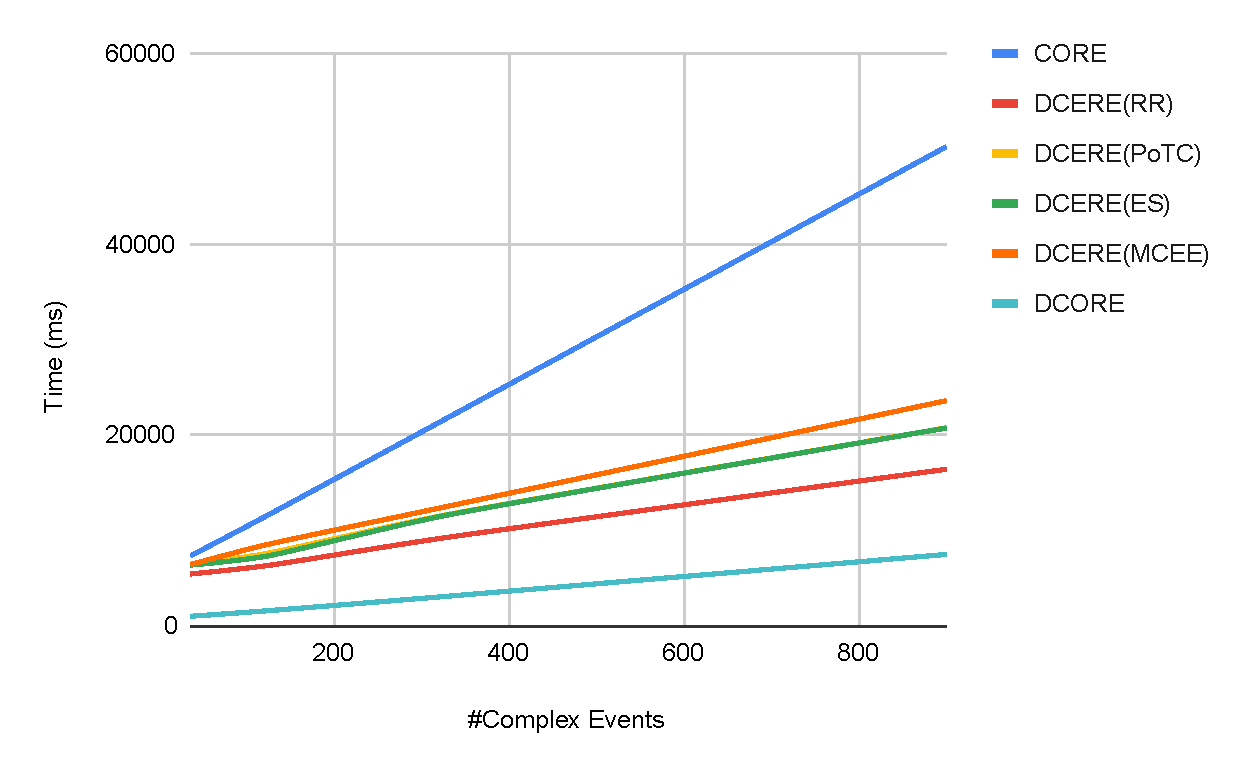
\includegraphics[width=\textwidth]{experiment_1_chart_1}
         \caption{$Q_{1}$}
         \label{fig:experiment:1:subfigure:1}
     \end{subfigure}
     \begin{subfigure}[b]{0.7\textwidth}
         \centering
         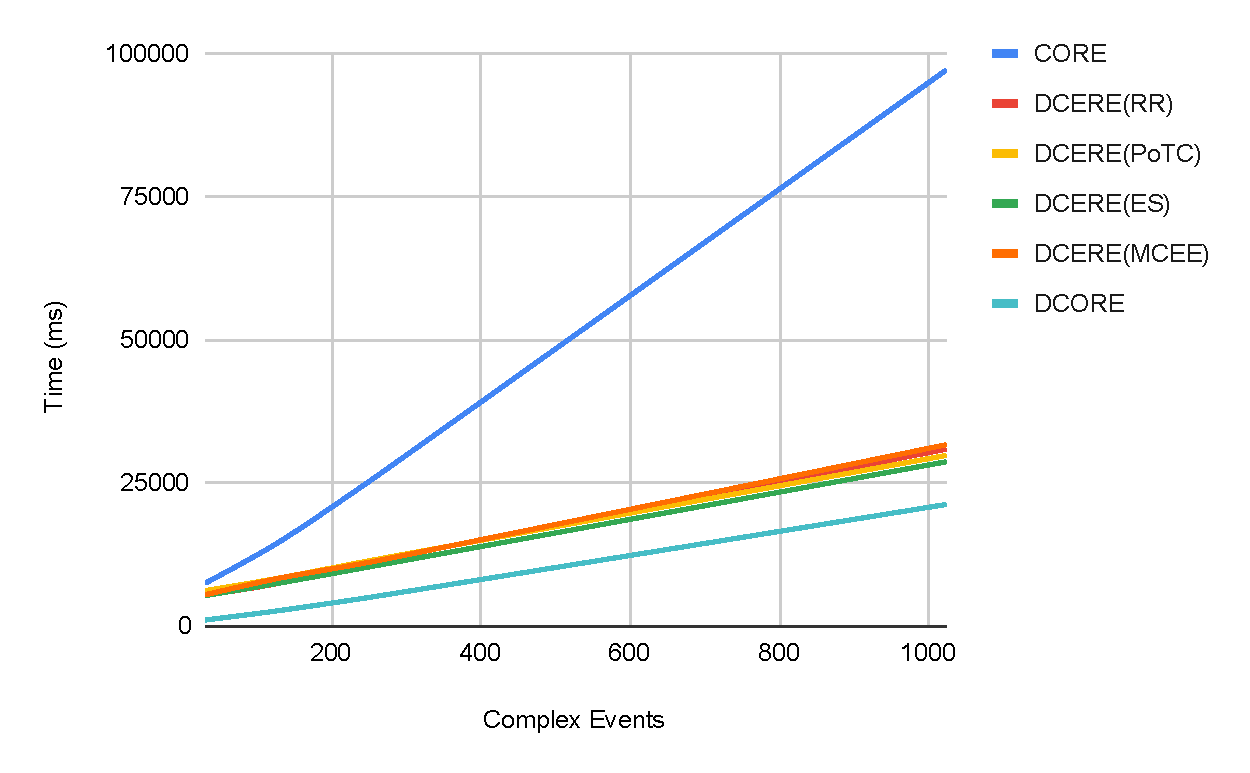
\includegraphics[width=\textwidth]{experiment_1_chart_2}
         \caption{$Q_{2}$}
         \label{fig:experiment:1:subfigure:2}
     \end{subfigure}
     \end{adjustbox}
     \begin{center}
      \begin{subfigure}[b]{0.7\textwidth}
          \centering
          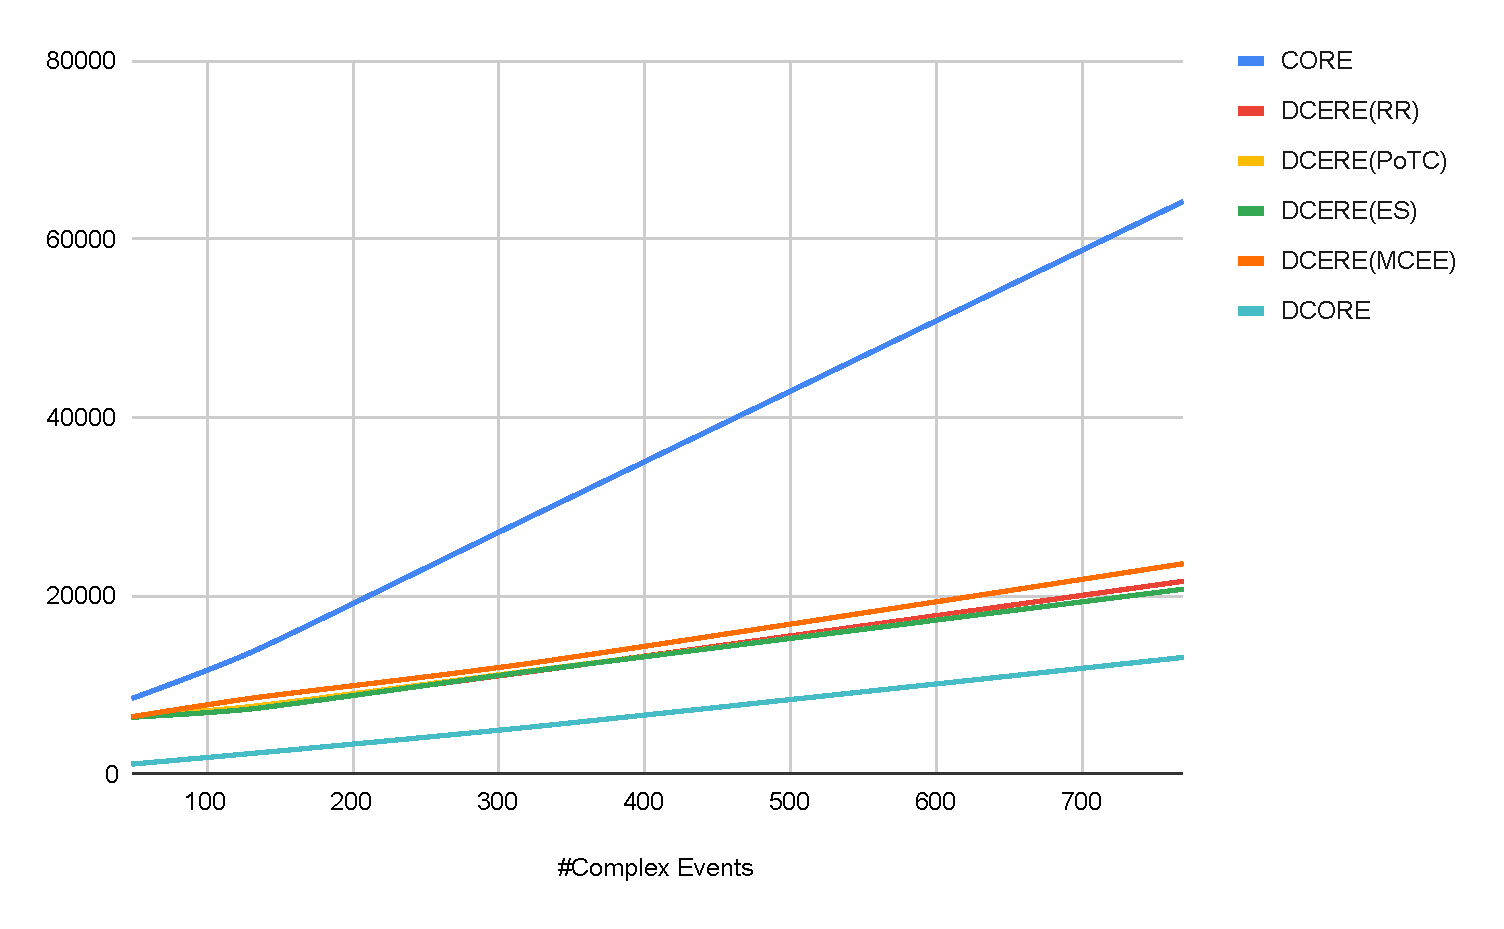
\includegraphics[width=\textwidth]{experiment_1_chart_3}
          \caption{$Q_{3}$}
          \label{fig:experiment:1:subfigure:3}
      \end{subfigure}
     \end{center}
     \caption{The performance of evaluating queries $Q_{1}$, $Q_{2}$, and $Q_{3}$ over stream $S_{1}$, $S_{2}$, $S_{3}$, respectively.}
     \label{fig:experiment:1}
\end{figure}

In this section, we designed an experiment to measure the performance characteristics of CORE, DCERE, and DCORE under queries with complex predicates. This experiment also evaluates the performance of DCERE under different distributions strategies. In Figure~\ref{fig:experiment:1}, we display the results of evaluating queries $Q_{1}$, $Q_{2}$, and $Q_{3}$ for an increasing number of complex events. The recognition time of all system increases as the number of complex event grows. Nevertheless, the degrading behaviour of CORE is more evident in this plot. Surprisingly, all distribution strategies have similar performance. The results of this experiment, validate our hypothesis that distribution strategy \emph{Maximal Complex Event Enumeration} does not perform well in practise, as discussed in Section~\ref{subsec:dcere:distribution-strategies}. We conclude that DCORE performs better than both CORE and DCERE. Furthermore, in the presence of complex and large streams, our novel distributed evaluation algorithm outperforms its sequential predecessor.

\section{Experiments on the scalability of the framework}\label{sec:scalability}

\begin{figure}[b]
     \begin{adjustbox}{max width=1.5\linewidth,center}
     \centering
     \begin{subfigure}[b]{0.45\textwidth}
         \centering
         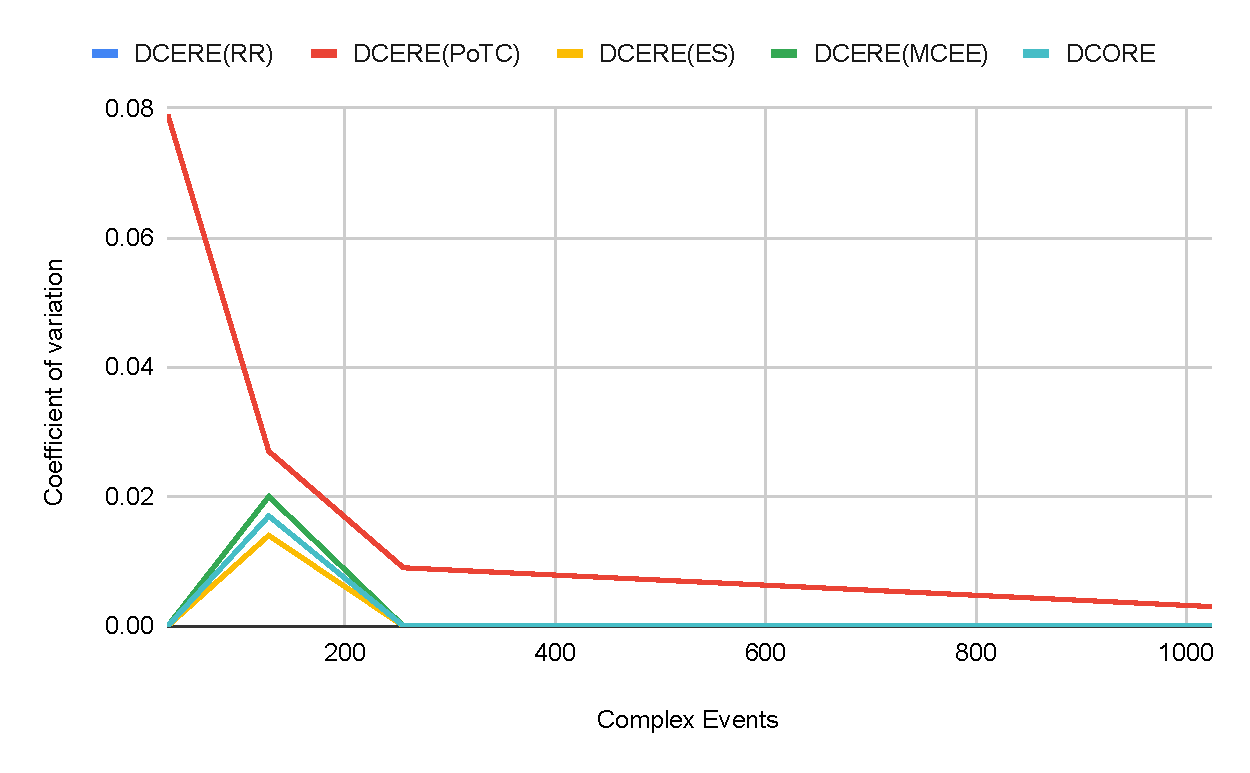
\includegraphics[width=\textwidth]{experiment_2_chart_1}
         \caption{$Q_{1}$}
         \label{fig:experiment:2:subfigure:1}
     \end{subfigure}
     \begin{subfigure}[b]{0.45\textwidth}
         \centering
         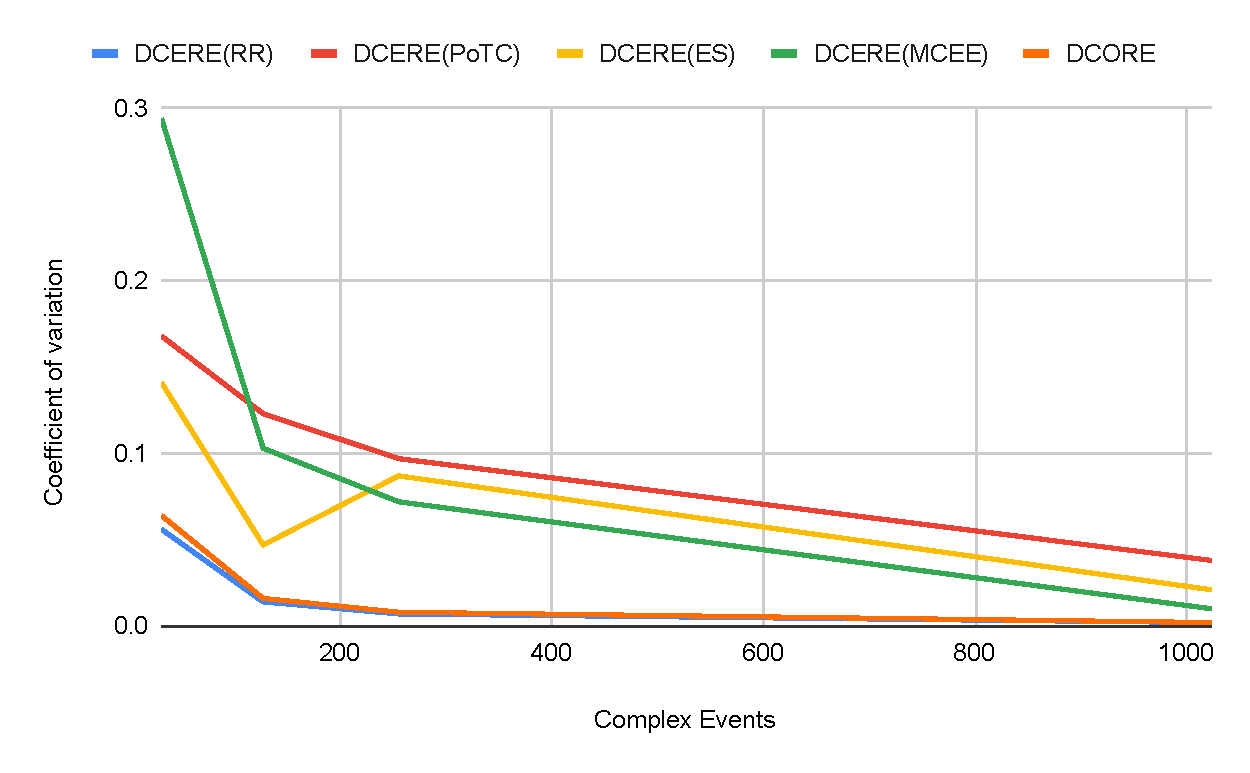
\includegraphics[width=\textwidth]{experiment_2_chart_2}
         \caption{$Q_{2}$}
         \label{fig:experiment:2:subfigure:2}
     \end{subfigure}
     \begin{subfigure}[b]{0.45\textwidth}
         \centering
         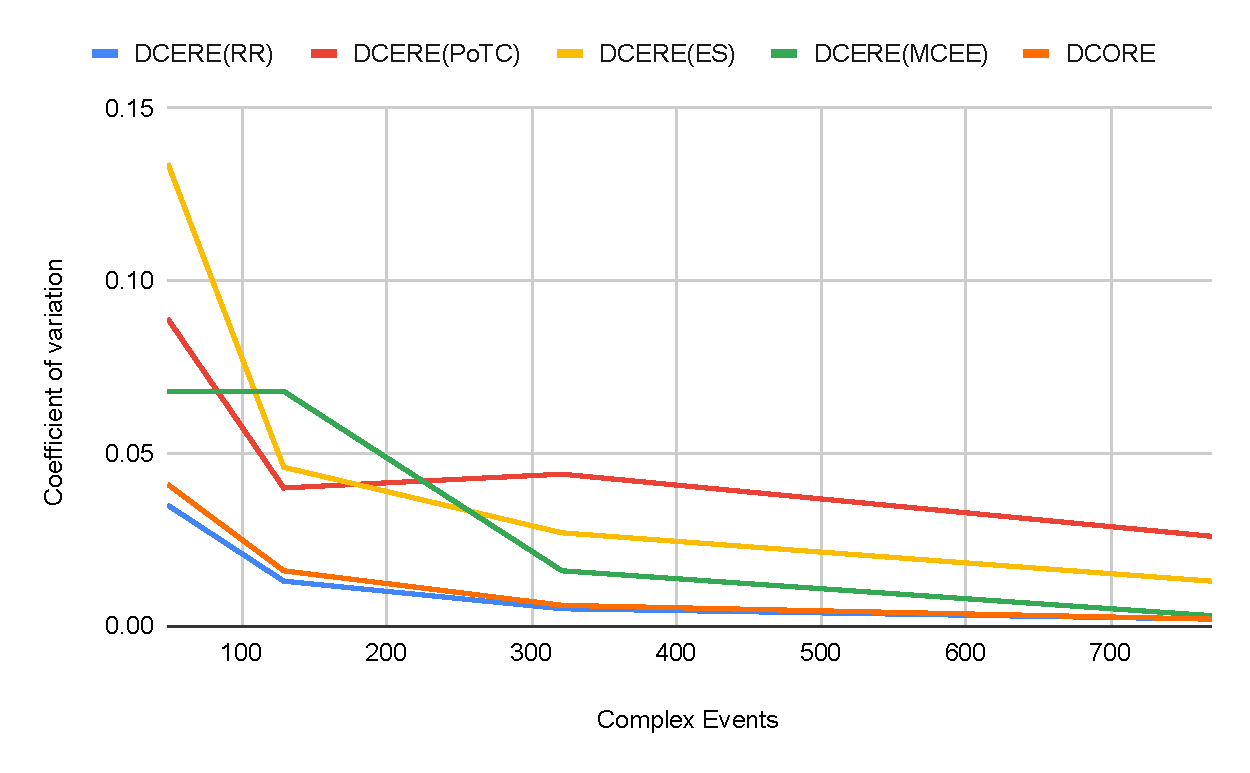
\includegraphics[width=\textwidth]{experiment_2_chart_3}
         \caption{$Q_{3}$}
         \label{fig:experiment:2:subfigure:3}
     \end{subfigure}
     \end{adjustbox}
     \caption{The coefficient of variation of evaluating queries $Q_{1}$, $Q_{2}$, and $Q_{3}$ under distributions strategies RR, PoTC, ES, and MCEE.}
     \label{fig:experiment:2}
\end{figure}

In this section, we study the scalability of DCERE and DCORE. For this reason, we designed two different experiments. The first experiment studies the quality on the load-balancing of the different distribution strategies, including DCORE. For this experiment, we compute the \emph{coefficient of variation} of the load of each processing unit during the evaluation of the queries $Q_{1}$, $Q_{2}$, and $Q_{3}$. The coefficient of variation (CV) is a standarized measure of \emph{dispersion} of a frequency distribution and it is defined as the ratio of the \emph{standard deviation} to the \emph{mean}. The lower the CV the less variability among the loads of the processing units; hence, a better scalability of the system on uniform processing units. In Figure~\ref{fig:experiment:2}, we show the coefficient of variation of the different distribution strategies (i.e. RR, PoTC, ES, and MCEE) and DCORE. The results show that all systems have a low coefficient of variation ($< 0.3$), with almost optimal CV on DCORE.

\begin{figure}[H]
     \begin{adjustbox}{max width=1.2\linewidth,center}
     \centering
     \begin{subfigure}[b]{0.7\textwidth}
         \centering
         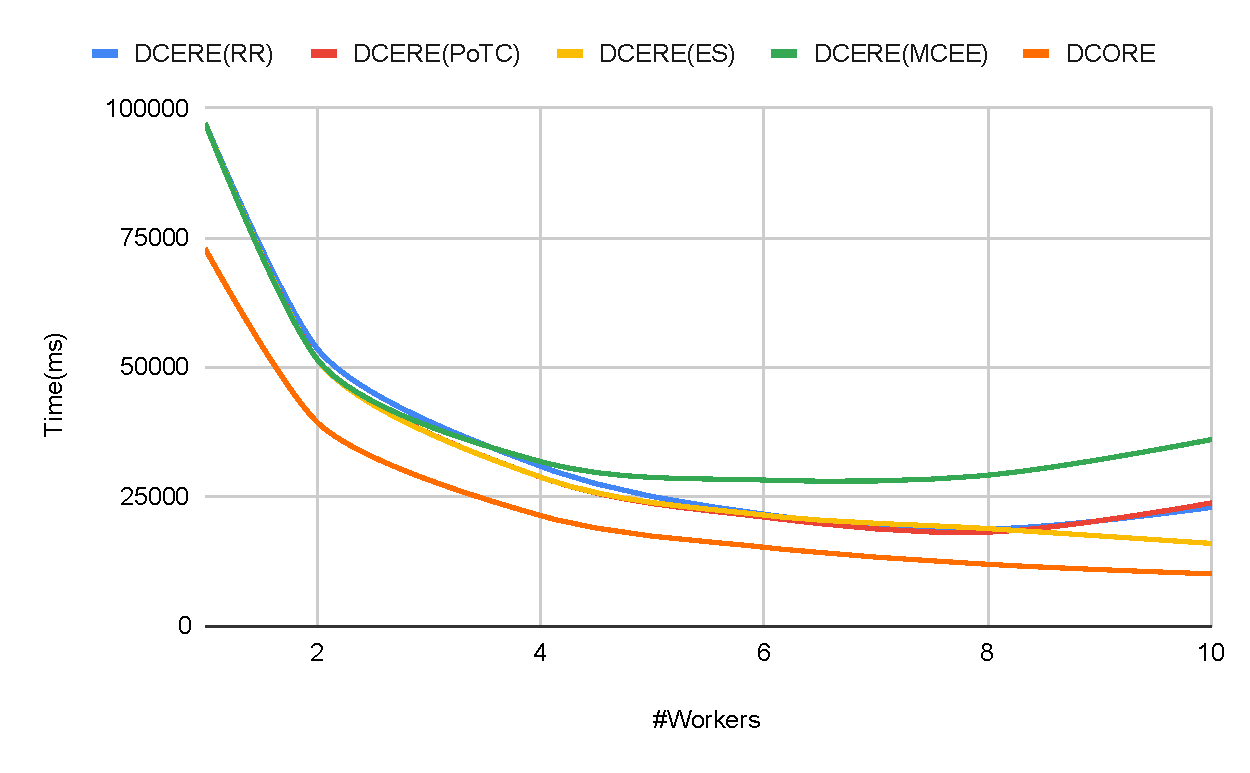
\includegraphics[width=\textwidth]{experiment_3_chart_1}
         \caption{$1024$ complex events}
         \label{fig:experiment:3:subfigure:1}
     \end{subfigure}
     \begin{subfigure}[b]{0.7\textwidth}
         \centering
         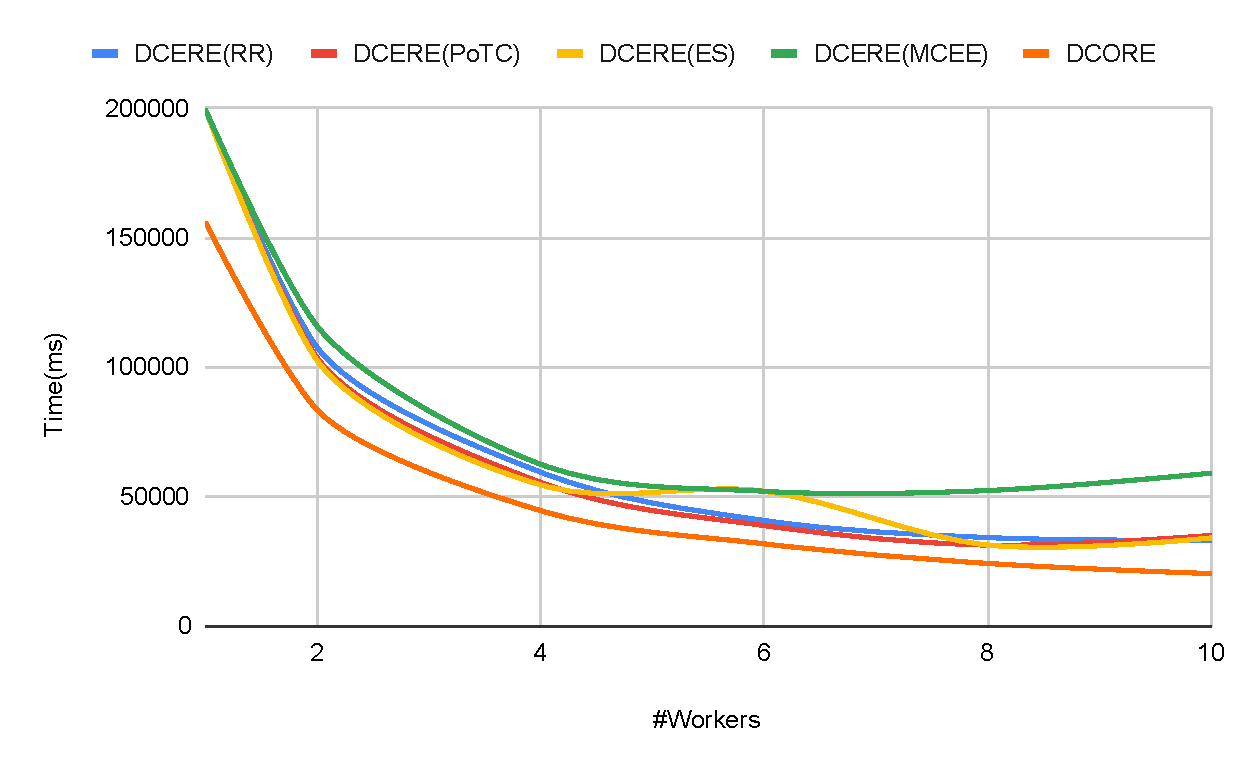
\includegraphics[width=\textwidth]{experiment_3_chart_2}
         \caption{$2048$ complex events}
         \label{fig:experiment:3:subfigure:1}
     \end{subfigure}
     \end{adjustbox}
     \caption{The horizontal scalability of DCERE and DCORE evaluating query $Q_{2}$ over increasing number of processing units.}
     \label{fig:experiment:3}
\end{figure}

The second experiment studies the horizontal scalability of the systems. In Figure~\ref{fig:experiment:3}, we show the execution time of the processing of query $Q_{2}$ on an increasing number of processing units (from $1$ to $10$). This experiment is run on two different streams. At the left, we executed the experiment with an stream that contained $1024$ complex events. At the right, the number of complex events is doubled, $2048$. This will allow us to study the impact of an increase of complexity in the scalability of the system. The results show that the system scales \emph{almost linearly} in the number of processing units until threshold $\tau$ of diminishing returns. DCERE's diminishing returns threshold is around $\tau = 8$, while DCORE's diminishing returns threshold is outside of the range of this experiment.

\section{Experiments on DCORE's evaluation algorithm under Big Data requirements}\label{sec:new-algorithm}

In this last section, we study the performance of the distributed evaluation algorithm of DCORE under heavy loads. For this reason, we designed three experiments. In the first experiment, we run DCORE over queries $Q_{1}$, $Q_{2}$, and $Q_{3}$, with variable number of processing units $1, 2, 4, 6, 8, 10$. For each configuration, we run the experiment on an increasing number of complex events. Notice, the number of complex events in this experiment is \emph{orders of magnitudes (OOM)} larger than in previous ones. In Figure~\ref{fig:experiment:4}, we show the execution time of the processing of queries $Q_{1}$, $Q_{2}$, and $Q_{3}$ under different number of processing units. The results show that under small loads, the sequential version of the algorithm (corresponding to DCORE with a single processing unit) performs better than the distributed version. Under heavy loads (i.e., more than 1 million complex events) the distribution pays off. The optimal number of processing units depend on the scale of the problem. For example, under a load of $10^{6}$ complex events the best configuration is 4 workers. We see that depending on the query, the performance of the system changes. We conclude that under small loads distributing the system only degrades performance, while under heavy loads the distribution speeds up the process of recognition of complex events.

\begin{figure}[t]
     \begin{adjustbox}{max width=1.3\linewidth,center}
     \centering
     \begin{subfigure}[b]{0.7\textwidth}
         \centering
         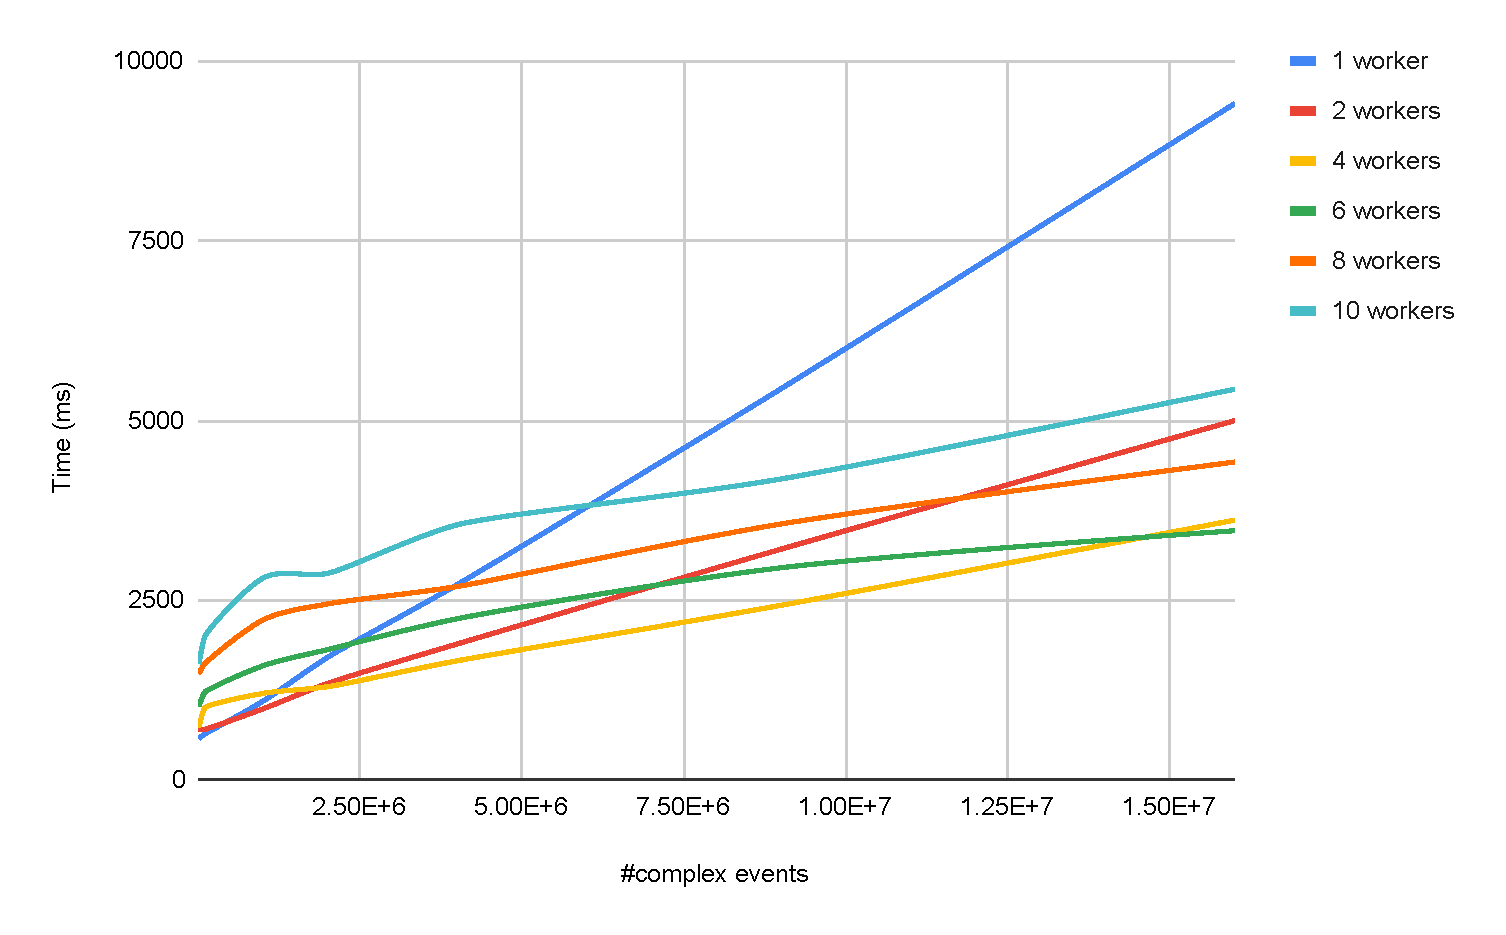
\includegraphics[width=\textwidth]{experiment_4_chart_1}
         \caption{$Q_{1}$}
         \label{fig:experiment:4:subfigure:1}
     \end{subfigure}
     \begin{subfigure}[b]{0.7\textwidth}
         \centering
         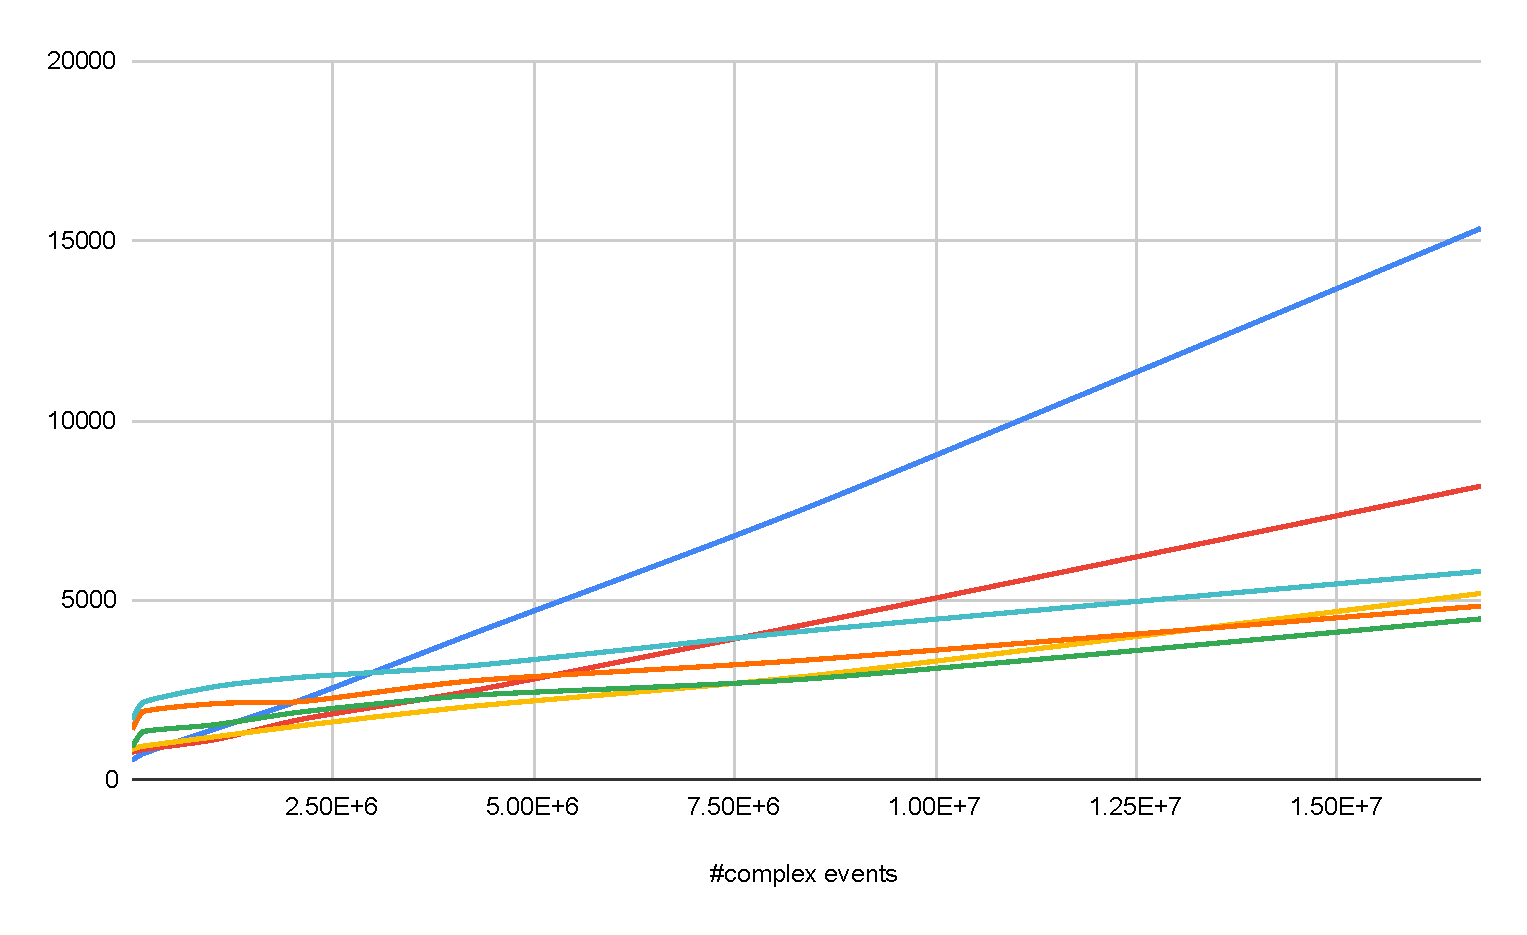
\includegraphics[width=\textwidth]{experiment_4_chart_2}
         \caption{$Q_{2}$}
         \label{fig:experiment:4:subfigure:2}
     \end{subfigure}
     \end{adjustbox}
     \begin{center}
     \begin{subfigure}[b]{0.7\textwidth}
         \centering
         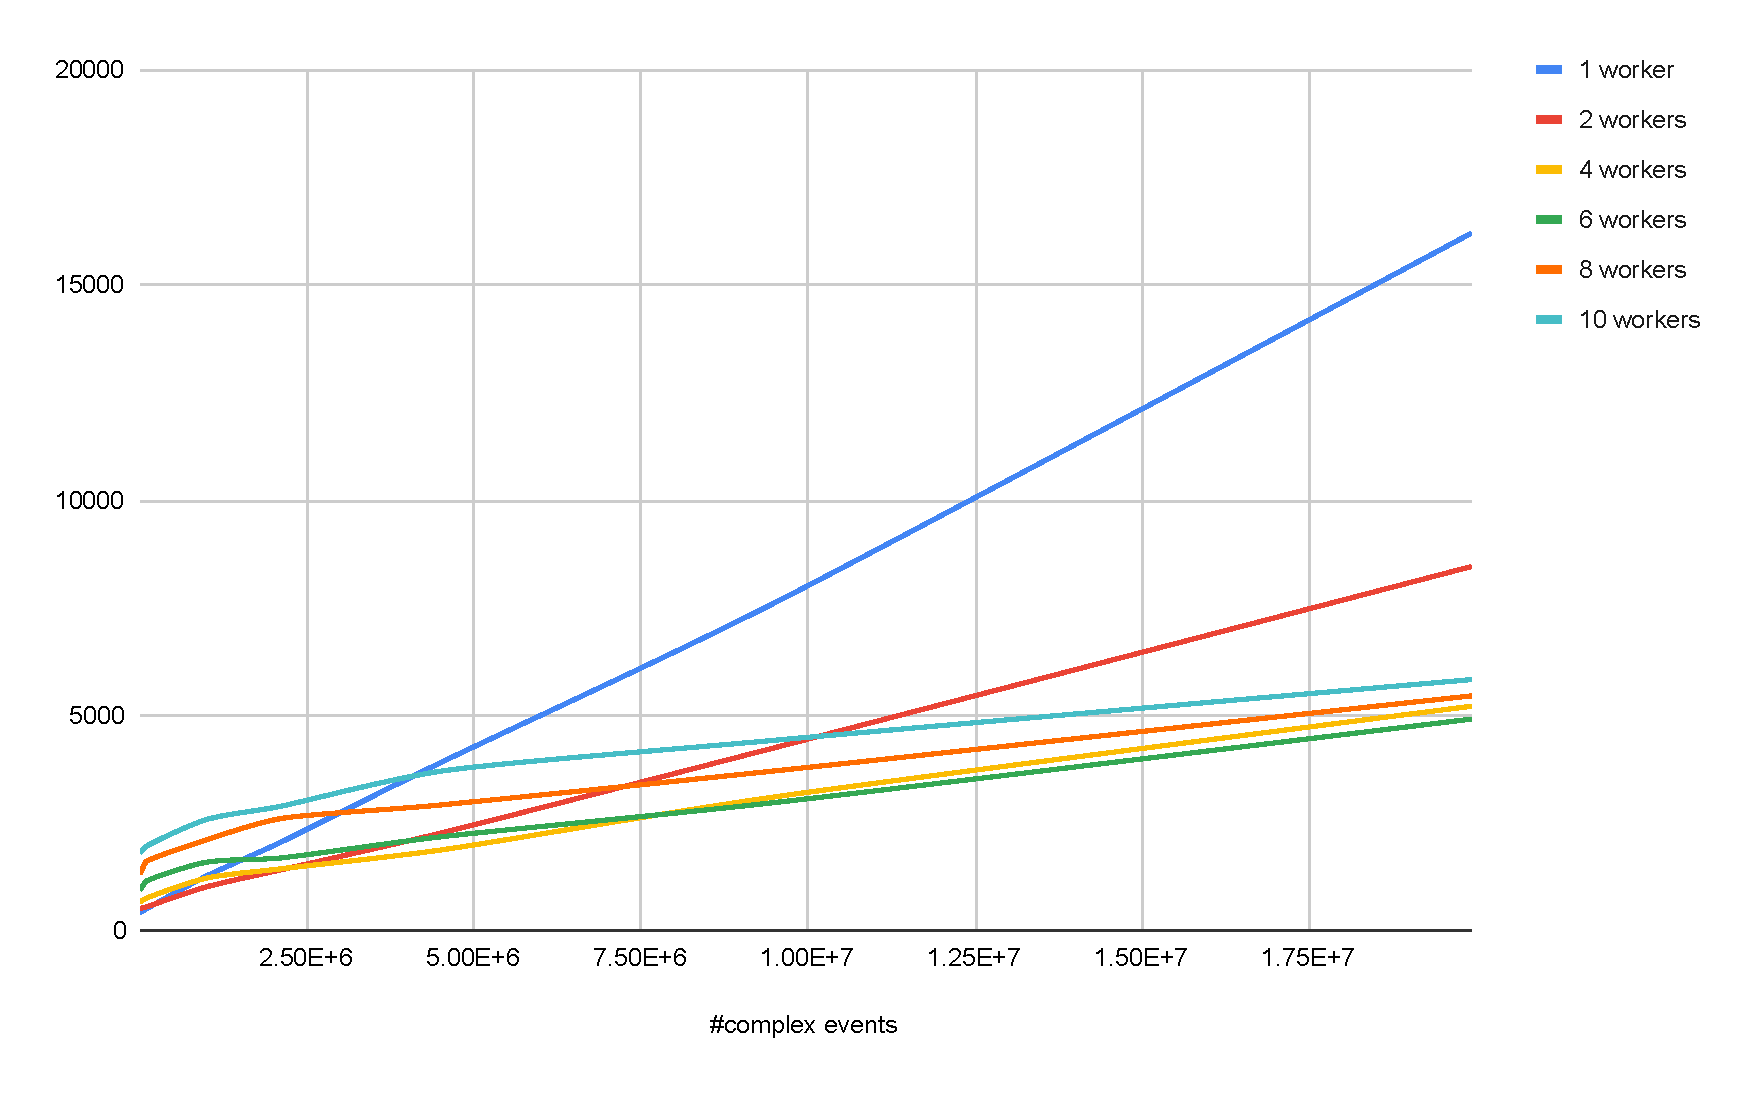
\includegraphics[width=\textwidth]{experiment_4_chart_3}
         \caption{$Q_{3}$}
         \label{fig:experiment:4:subfigure:3}
     \end{subfigure}
     \end{center}
     \caption{The horizontal scalability of DCORE under increasing number of processing units.}
     \label{fig:experiment:4}
\end{figure}

In the second experiment, we study the execution time of each processing unit during the evaluation of queries $Q_{1}$, $Q_{2}$, and $Q_{3}$. The goal of this experiment is to analyse the amount of work of each processing unit. A balanced distribution of work loads would result in overall better performance of the system. In Figure~\ref{fig:experiment:5}, we show the results of the second experiment on $8$ processing units over a fixed length of stream. The results show no evidence of significant differences between the execution time on each processing unit. We conclude that this is a relevant factor on the performance of DCORE.

\begin{figure}[t]
  \centering
  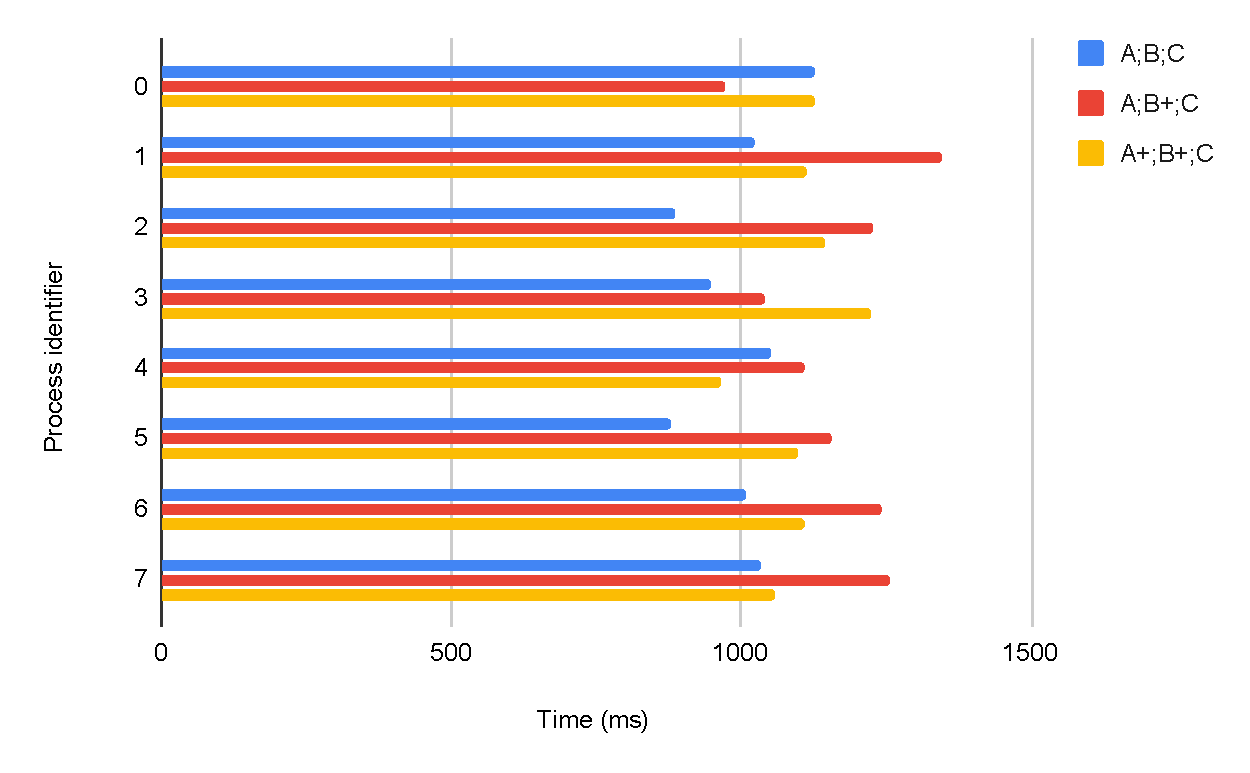
\includegraphics[scale=0.5]{experiment_5_chart_1}
  \caption{The execution time on each processing unit of DCORE evaluating queries $Q_{1}$, $Q_{2}$, and $Q_{3}$.}
  \label{fig:experiment:5}
\end{figure}

\begin{figure}[H]
     \begin{subfigure}[b]{0.49\textwidth}
         \centering
         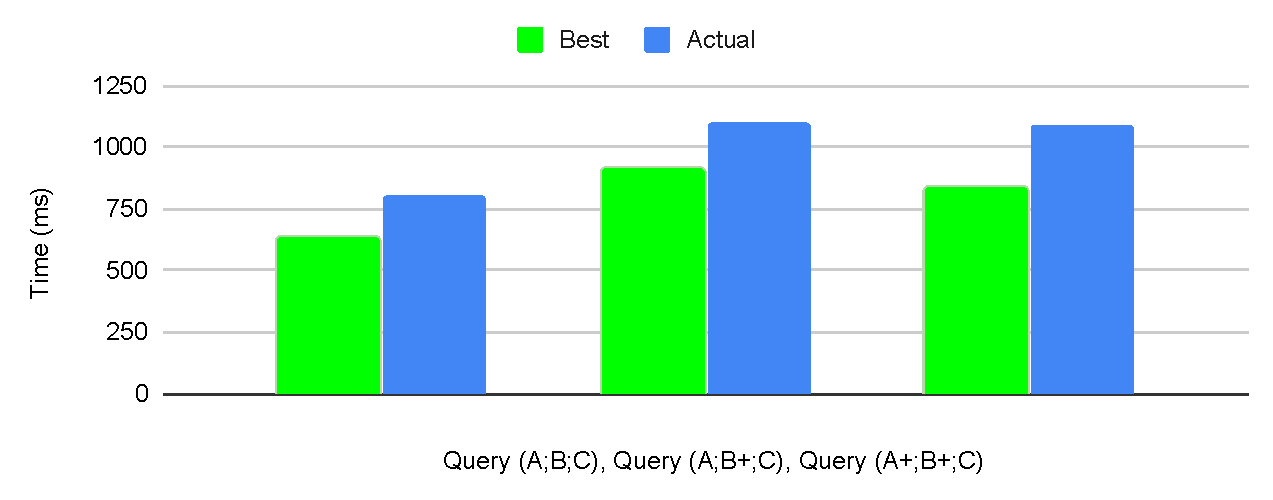
\includegraphics[width=\textwidth]{experiment_5_chart_2}
         \caption{$2$ processes}
         \label{fig:experiment:6:subfigure:1}
     \end{subfigure}
     \begin{subfigure}[b]{0.49\textwidth}
         \centering
         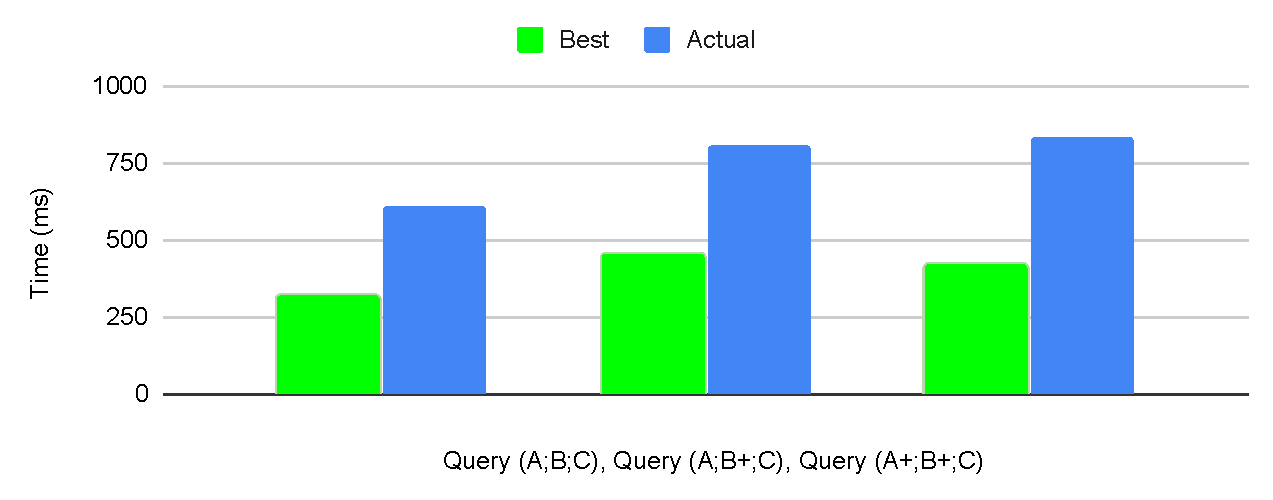
\includegraphics[width=\textwidth]{experiment_5_chart_3}
         \caption{$4$ processes}
         \label{fig:experiment:6:subfigure:2}
     \end{subfigure}
     \begin{subfigure}[b]{0.49\textwidth}
         \centering
         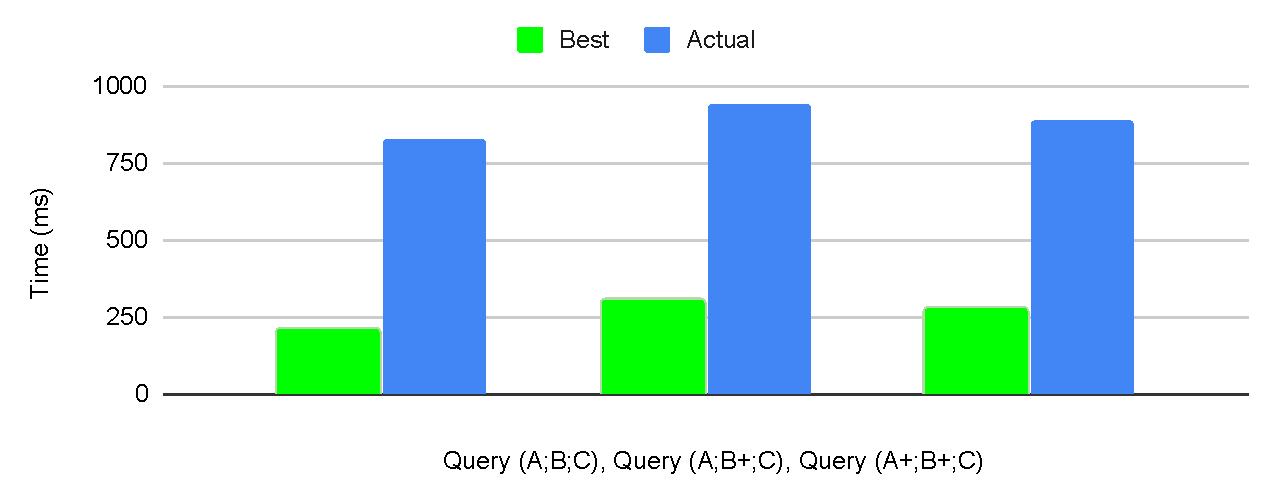
\includegraphics[width=\textwidth]{experiment_5_chart_4}
         \caption{$6$ processes}
         \label{fig:experiment:6:subfigure:3}
     \end{subfigure}
     \begin{subfigure}[b]{0.49\textwidth}
         \centering
         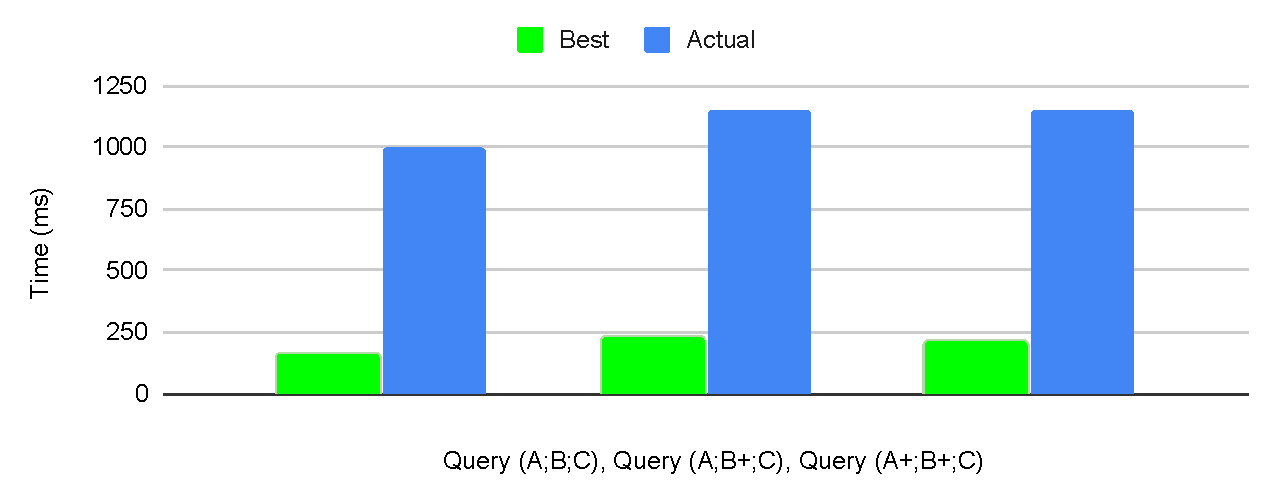
\includegraphics[width=\textwidth]{experiment_5_chart_5}
         \caption{$8$ processes}
         \label{fig:experiment:6:subfigure:4}
     \end{subfigure}
     \caption{Comparison of the execution time of an optimal distributed system based on CORE against DCORE.}
     \label{fig:experiment:6}
\end{figure}

In this last experiment, we compare the performance of DCORE against an hypothetical optimal distributed system based on CORE. The goal of this experiment is to analyse how close is DCORE from an optimal distributed system with same performance characteristics on the evaluation algorithm (e.g., CORE). For this experiment, we evaluated queries $Q_{1}$, $Q_{2}$, and $Q_{3}$ over a stream of fixed length that produced $2 \cdot 10^{6}$ complex events. The experiment is repeated for different number of processes: $2, 4, 6, 8$. In Figure~\ref{fig:experiment:6}, we show the results of this experiment. The blue bars corresponds to the execution time of the experiment for DCORE, while the green bars corresponds to the execution time of CORE divided by the number of processing units of each iteration, which hypothetically corresponds to the best performance DCORE could ever achieve. The results show that DCORE is close to the optimal value when distributed over 2 processing units. However, the gap grows as the number of processing units increases. We conjecture that the cost of enumerating the first complex event in the data structure diminish the performance gains from distributions. In other words, in order to compensate the cost of enumerating the first path on the tECS, which is linear in the size of the complex event, each processing unit requires a reasonable amount of complex events.

\section{Chapter summary}

In this chapter, we presented a set of experiments to study the performance and scalability of both our distributed framework for CER and our distributed evaluation algorithm. First, we describe the implementation of DCORE. Then, we described the general settings of the experiments such as hardware, input streams and queries, among others. Finally, we presented and discussed the experiments, and their corresponding results.
